\section{Heur\'istica constructiva golosa}

Para la heur\'istica constructiva golosa tenemos en cuenta como cada ``paso'' de la heu\'istica el colocar un nodo del grafo en alguna
de las $k$ particiones, como elecci\'on candidata cada una de las $k$ particiones donde puede colocarse el nodo y como ``soluci\'on local'' de
cada paso el conjunto que tiene por resultado el peso m\'inimo. \\\

Consideremos la siguiente instancia del problema como ejemplo, con $k=2$:
\begin{figure}[h!]
  \centering
  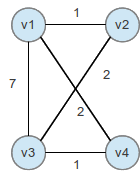
\includegraphics[width=0.25\textwidth]{ej3/greedy_graph_example1.png}
  \caption{Instanca de un problema 2-PMP}
\end{figure}

\begin{figure}[H]
        \centering
        \begin{subfigure}[b]{0.25\textwidth}
                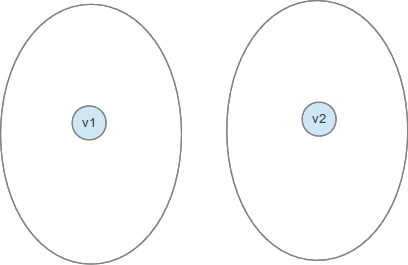
\includegraphics[width=\textwidth]{ej3/greedy_graph_partition_example1.png}
                \caption{Estado de la soluci\'on luego de las dos primeras elecciones.}
                \label{fig:greedy_fig_2}
        \end{subfigure}%
         \qquad
         \qquad
         \qquad
         \qquad
         \qquad
         %add desired spacing between images, e. g. ~, \quad, \qquad, \hfill etc.
          %(or a blank line to force the subfigure onto a new line)
        \begin{subfigure}[b]{0.25\textwidth}
                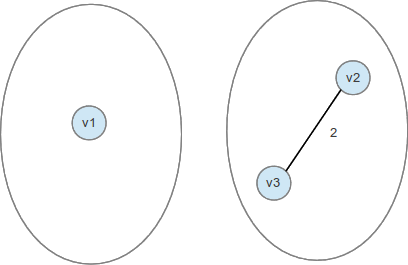
\includegraphics[width=\textwidth]{ej3/greedy_graph_partition_example2.png}
                \caption{Estado de la soluci\'on luego de la tercera elecci\'on.}
                \label{fig:greedy_fig_3}
        \end{subfigure}
        \caption{Ejecuci\'on del algoritmo greedy paso por paso.}
        \label{greedy_algorith_example1}
\end{figure}

Como puede observarse dado un grafo el algoritmo considera un posible orden de sus vertices $v_{1}, \ldots, v_{n}$ (notemos que la elecci\'on de este \'orden es
arbitraria y depende de la implementaci\'on) y comienza a colocarlos en cada una de las $k$ particiones del problema de forma secuencial, intentando
minimizar el peso en cada elecci\'on. \\
En cada paso de la generaci\'on de la soluci\'on final la elecci\'on de ese paso solo
tiene en cuenta las aristas que unen al nuevo nodo que todav\'ia no forma parte de la soluci\'on con los nodos que fueron agregados a la soluci\'on
en el paso anterior. Es inmediato observar que utilizando este algoritmo se pierde de analizar posibles combinaciones de nodos en las particiones por
lo que podr\'ia no alcanzarse la soluci\'on \'optima. \\\

En el ejemplo anterior:
\begin{figure}[h!]
  \centering
  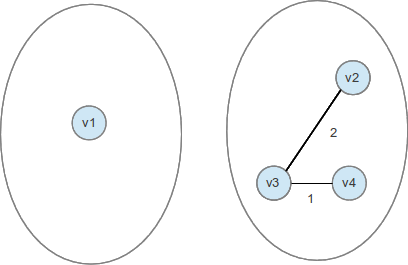
\includegraphics[width=0.4\textwidth]{ej3/greedy_graph_partition_example3.png}
  \caption{Soluci\'on obtenida mediante el algoritmo goloso, $\omega = 3$.}
\end{figure}

\begin{figure}[h!]
  \centering
  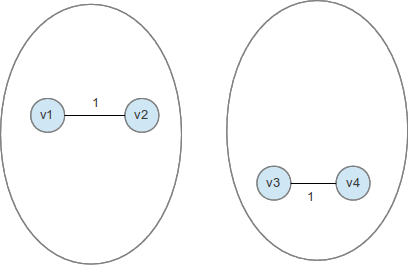
\includegraphics[width=0.4\textwidth]{ej3/greedy_graph_partition_example4.png}
  \caption{Soluci\'on \'optima del problema, $\omega = 2$.}
\end{figure}



\subsection{Algoritmo}


\begin{algorithm}[H]
 \KwData{$G=(V,E), \,k:int$}
 \KwResult{$particiones: V_{1}, \ldots, V_{k} , \,  weight: int$ }
	$V_{1}, \ldots , V_{k} = \emptyset$\;
	\For{$v = v_{1}, \ldots , v_{n} \in V$}{
		$i:$ Tal que $\omega(V_{i}) = min(\{ \omega(V_{j} \bigcup \{v\})$ / $ 1 \leq j \leq k \})$\;
		$V_{i} = V_{i} \bigcup \{v\}$\;
   	}   	
	\Return {$<V_{1}, \ldots, V_{k}, \omega(V_{1}) + \ldots + \omega(V_{k})>$}
\caption{Heur\'istica constructiva golosa k-PMP\label{alg_ej3}}  
\end{algorithm} 

\subsubsection{An\'alisis de complejidad}
Observemos que el ciclo de la l\'inea 2 realiza una iteraci\'on por cada uno de los nodos del grafo, teniendo complejidad $O(n)$ por la complejidad
del cuerpo del ciclo. La l\'inea 4 puede realizarse en tiempo $O(1)$ (dependiendo de la estructura utilizada para representar las particiones).
Por \'ultimo la l \'inea 3 tiene c\'alcular el m\'inimo de la suma de los pesos de las aristas, de agregar el nuevo nodo a cada una de loas particiones.
Esto no es m\'as que realizar la suma del nuevo nodo contra las aristas que forman parte de cada una de las particiones y puede hacerse en tiempo
$O(km)=O(kn^{2})$. \\\
En definitiva sea $T(n)$ la funci\'on de costo del algoritmo goloso, $T(n) \in O(kn^{3})$.

\subsubsection{An\'alisis de las soluciones obtenidas}
Volviendo a la observacion que realizamos antes, un problema del algoritmo goloso es que no tiene en cuenta al momento de tomar decisiones las aristas
de los nodos que todav\'ia no forman parte de la soluci\'on. \\\

Observemos el siguiente caso con $ 2 \leq k \leq 4$:
\begin{figure}[H]
  \centering
  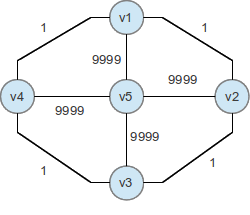
\includegraphics[width=0.4\textwidth]{ej3/greedy_graph_star+cicle_example1.png}
  \caption{Instancia ``estrella + ciclo''.}
\end{figure}

Es inmediato ver que si el algoritmo procesa secuencialmente los nodos $v_{1}, \ldots ,v_{5}$, los 4 primeros nodos quedaran distribuidos entre las $k$
particiones y el nodo $v_{5}$ arruinara el resultado con alguna de sus aristas de peso $9999$. Para llegar a la soluci\'on \'optima es aislar al
nodo del centro en una partici\'on y luego distribuir el resto en las particiones restantes. 

\begin{figure}[H]
        \centering
        \begin{subfigure}[b]{0.7\textwidth}
                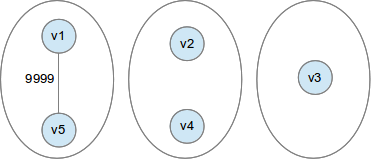
\includegraphics[width=\textwidth]{ej3/greedy_graph_star+cicle_partition_example1.png}
                \caption{Soluci\'on obtenida mediante el algoritmo goloso, $\omega(S) = 9999$.}
                \label{fig:greedy_fig_3}
        \end{subfigure}%
         \qquad
         \qquad
         \qquad
         \qquad
         \qquad
         %add desired spacing between images, e. g. ~, \quad, \qquad, \hfill etc.
          %(or a blank line to force the subfigure onto a new line)
        \begin{subfigure}[b]{0.7\textwidth}
                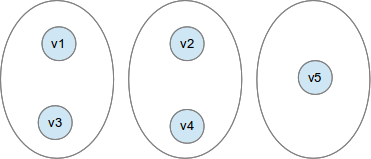
\includegraphics[width=\textwidth]{ej3/greedy_graph_star+cicle_partition_example2.png}
                \caption{Soluci\'on \'optima del problema, $\omega(S) = 0$.}
                \label{fig:greedy_fig_4}
        \end{subfigure}
        \caption{Ejecuci\'on del algoritmo greedy paso por paso.}
        \label{greedy_algorith_example2}
\end{figure}

Esta idea puede generalizarse demostrando que el resultado propuesto por la her\'istica golosa puede ser arbitrariamente malo dependiendo del grafo. Cualquier
grafo que tenga una componente ``ciclo simple de tama\~no $n-1$'' $\bigcup$ ``estrella de tama\~no $n$'', donde el peso de las aristas de la estrella $L > \omega(e_{1}) + \ldots + \omega(e_{n-1})$, es decir
mayor a la suma de los pesos de todas las aristas del ciclo. De esta manera aun tratando una instancia del problema k-PMP donde $k=2$ resulta conveniente para minimizar el peso de la componente  aislar ç
el nodo de la estrella y agrupar todos los nodos del ciclo en una misma partici\'on. \\
Debido a la implementaci\'on de la heur\'istica golosa que utiliza \'orden lexicografico, si el nodo central de la estrella es el \'ultimo en ser considerado, nunca se tendran en cuenta las aristas
m\'as pesadas para decidir aislar este nodo.

\begin{figure}[H]
  \centering
  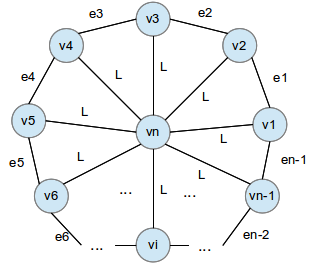
\includegraphics[width=0.4\textwidth]{ej3/greedy_graph_star+cicle_example2.png}
  \caption{Instancia ``estrella + ciclo'' de tamaño n.}
\end{figure}
  
\subsection{Experimentaci\'on}
